\begin{figure}
    \centering
    \subfloat[Skew verses eigengap]{%
        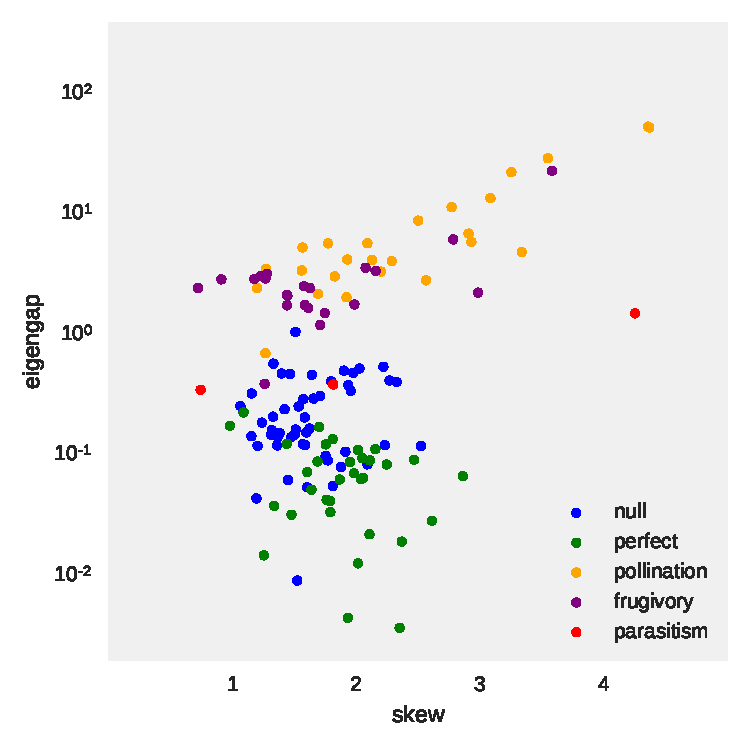
\includegraphics[width=0.5\textwidth]{figures/codiv_literature_skew_eigengap.pdf}
    }
    \subfloat[Hierarchical clustering by distance]{%
        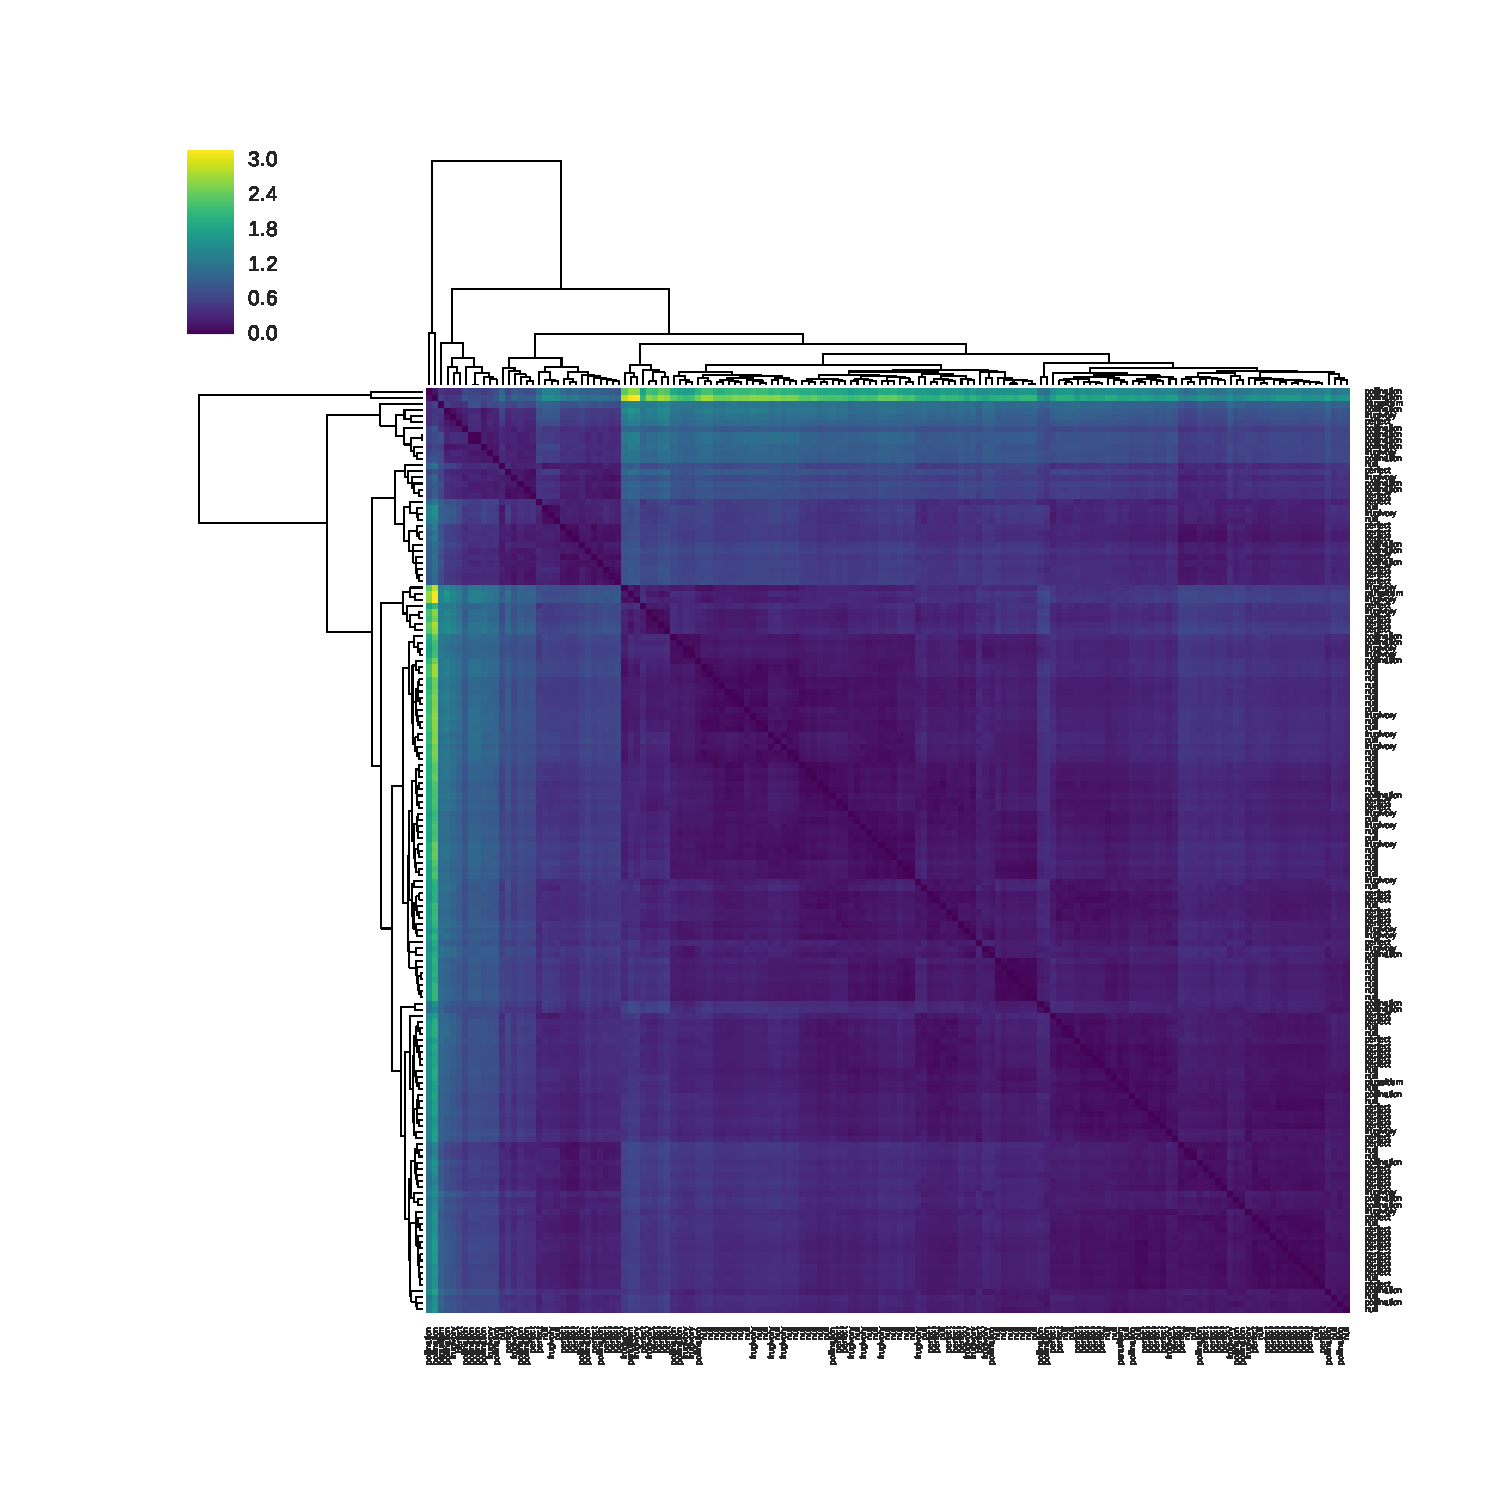
\includegraphics[width=0.5\textwidth]{figures/codiv_literature_clustermap.pdf}
    }
    \caption{Spectral properties of examples of co-diversification gathered from the literature and simulated cases of independent and parallel diversification. The spectral distributions of these graphs can be separated into different groups either by extracting summary statistics, such as their skew and eigengap \textbf{(a)}, or by hierarchical clustering of their pairwise Shannon-Jensen distances \textbf{(b)}.}
    \label{fig:FP_codivlit}
\end{figure}